\documentclass[a4paper]{article}
\usepackage[pdftex]{graphicx}
\usepackage{anysize}
\marginsize{3cm}{3cm}{3cm}{3cm}
\linespread{1.2}
\usepackage[utf8]{inputenc}
\usepackage[T1]{fontenc}       
\usepackage[swedish]{babel}      
\usepackage{epstopdf}     % För svensk avstavning och svenska
\usepackage[osf]{mathpazo} % Palatino with smallcaps and oldstyle numbers
\usepackage[scaled]{helvet}
\usepackage{float}
\restylefloat{table}
\usepackage{etoolbox}

\newcommand\getcurrentref[1]{%
 \ifnumequal{\value{#1}}{0}
  {??}
  {\the\value{#1}}%
}  
\newcommand\requirement[2]{
	\numberedrow{Krav}{#1}{#2}
}
\newcommand\scenario[2] {
	\numberedrow{Scenario}{#1}{#2}
}
\newcommand\numberedrow[3]{
	\noindent
	\textbf{#1 \getcurrentref{section}.\getcurrentref{subsection}.#2.} #3
	
}

\usepackage{fancyhdr}
\fancyhf{}
\fancyhead[L]{Ansvarig: SG}

\fancyhead[R]{Datum: \today | Version: 0.18 | Dokumentnummer: PUSS144401}


\title{SRS - Software Requirements Specification: NewPussSystem}                  	
\author{Systemarkitektgruppen \\ Lars Gustafsson | Martin Lichota | Marcel Tovar Rascon}
\date{}

\begin{document}

\maketitle
\thispagestyle{fancy}
\tableofcontents
\newpage

\section*{Dokumenthistorik}

\begin{tabular}{ l l l p{8.5cm} }
Ver. & Datum & Ansv. & Beskrivning \\\hline
0.1 & 8 september 2014 & SG & Struktur för dokumentet\\
0.2 & 10 september 2014 & SG & Lägga till krav från UG\\
0.3 & 11 september 2014 & SG & Revidera krav samt ändra struktur\\
0.4 & 12 september 2014 & SG & Lade till nya samt reviderade krav\\
0.5 & 12 september 2014 & SG & Lade till nya samt reviderade krav\\
0.6 & 12 september 2014 & SG & Lade till nya samt reviderade krav\\
0.7 & 12 september 2014 & SG & Lade till nya samt reviderade krav\\
0.8 & 12 september 2014 & SG & Lade till nya samt reviderade krav\\
0.9 & 12 september 2014 & SG & Reviderade krav samt lade till scenarion\\
0.10 & 13 september 2014 & SG & Skapade scenarion för projektledning.\\
0.11 & 13 september 2014 & SG & Skapade scenarion för tidrapportmall och lade till krav.\\
0.12 & 14 september 2014 & SG & Administration och tidrapportering är klart.\\
0.13 & 14 september 2014 & SG & Lade till kontextdiagram samt uppdaterade krav under områdena projektledning, kvalitet och projekt.\\
0.14 & 15 september 2014 & SG & 

Uppdaterat efter granskningsprotokoll från TG, UG, och intern gransking i SG.
Uppdaterat formuleringar, kapitel \ref{bom-aktorer} och \ref{terminologi}. 
Uppdaterat krav, kapitel \ref{krav-funk-gen}, \ref{krav-funk-aut}, \ref{krav-funk-data}, \ref{krav-funk-admin}, \ref{krav-funk-tid}.
Lagt till nya krav, kapitel \ref{krav-funk-data}, \ref{krav-funk-admin}, \ref{krav-funk-tid}.
Uppdaterat scenario, kapitel \ref{krav-funk-proj}. \\
0.15 & 16 september 2014 & SG & Uppdaterade design och lade till formulering, kapitel \ref{terminologi}.
Lade till krav, kapitel \ref{krav-funk-data}.
Uppdaterade krav, kapitel \ref{krav-funk-proj}, \ref{krav-kval-pres}.\\
0.16 & 16 september 2014 & SG & Tog bort reduntant krav, kapitel \ref{krav-funk-data}.
Lade till krav, kapitel \ref{krav-funk-data}\\
0.17 & 16 september 2014 & SG & Ändrat krav \ref{krav-funk-data}.18, \ref{krav-funk-data}.19, scenario \ref{krav-funk-admin}.4, scenario \ref{krav-funk-admin}.1 och scenario \ref{krav-funk-admin}.3. Lagt till krav \ref{krav-funk-admin}.21, \ref{krav-funk-admin}.22 och scenario \ref{krav-funk-admin}.5.
\\
0.18 & 21 september 2014 & SG & Revidering efter formell granskning.\\

\\
\end{tabular}
\section{Inledning}       
Dokumentet beskriver kraven för NewPussSystem, ett tidrapportingssystem för projekt som diverse användare kan logga in på.

\section{Referensdokument}
I denna version används inget referensmaterial.
\section{Bakgrund och mål}   
\subsection{Huvudmål}
Huvudmålet är att tillhandhålla ett system där olika användare, såsom projektledare och övriga projektmedlemmar, skall kunna tidrapportera och loggföra det fortgående arbetet i sitt projekt. 

\subsection{Aktörer och deras mål}
\label{bom-aktorer}
Följande aktörer kommer att använda systemet:
\begin{itemize}
\item [] \textbf{Vanlig användare} En vanlig användare är en person med ett konto i systemet som ännu inte har blivigt tilldelad ett projekt.
\item [] \textbf{Projektmedlem(t1, t2, t3)} En vanlig användare kan tilldelas rollen som projektmedlem. Denne kan tidrapportera och har även tillgång till historik rörande den egna samt gruppens totala tidrapportering. T1, t2, och t3 indikerar tre olika projektmedlemsroller, en användare blir tilldelad en av dessa i samband med att den blir medlem i ett projekt.
\item [] \textbf{Projektledare} En användare kan tilldelas rollen som projektledare vilket ger den administrativa rättigheter för ett givet projekt. En projektledare kan tillsätta vanliga användare en projektmedlemsroll. Utöver sina rättigheter som projektledare har den all funktionallitet som en projektmedlem besitter.
\item [] \textbf{Administratör} En administratör är en och endast en användare som har befogenheter att lägga till och ta bort andra användare. Administratören tillsätter även projektledare och skapar projektgrupper. Administratören kan inte deltaga i en projektgrupp men har utöver detta samma priviligerade rättigheter som projektledare coh projektmedlem.
\end{itemize}
\section{Terminologi}
\label{terminologi}
Här följer ord och uttryck som används i rapporten och är till för att öka förståelsen.
\begin{itemize}
\item []\textbf{Användarnamn:} Unik indentifikationsfras för att representera en användare i systemet..
\item []\textbf{Lösenord:} Hemlig fras endast känd för var unik användare samt systemet så användaren kan påvisa sin identitet.
\item []\textbf{Logga:} in Då en användare identifierar sig mot systemet med användarnamn och lösenord, om systemet godkänner identifieringen loggar användaren in.
\item []\textbf{Inloggad:} En användare som har loggat in är inloggad.
\item []\textbf{Användarstatus:} En indikation på var användare som avgör hur vida den får logga in eller ej.
\item []\textbf{Projektgrupp:} En grupp bestående av projektmedlemmar och projektledare.
\item []\textbf{Tidrapport:} En rapport som innehåller arbetsbelasting för en användare under en fix tidperiod bundet till en specefik projektgrupp.
\item []\textbf{Huvudsida:} Med huvudsida avses den första vyn som användaren blir dirigerad till direkt efter inloggning. 
\item []\textbf{Användarlista:} En lista med alla användarnamn och lösenord som är sparade i databasen.
\item []\textbf{Aktivitetsruta:} Cellen där aktivitet (raden) och subaktivitet (kolumnen) möts.
\item []\textbf{Information:} Med information avses t.ex. användare, projekt eller tidrapporter.
\item []\textbf{FIFO:} Från engelskans first in first out. Teknik som fungerar på samma sätt som en kö. Den som kom först betjänas först.

\end{itemize}
\section{Kontextdiagram}
Kontextdiagram för NewPussSystem illustreras av Figur \ref{image_kontext}.

\begin{figure}[h!]
  \centering
    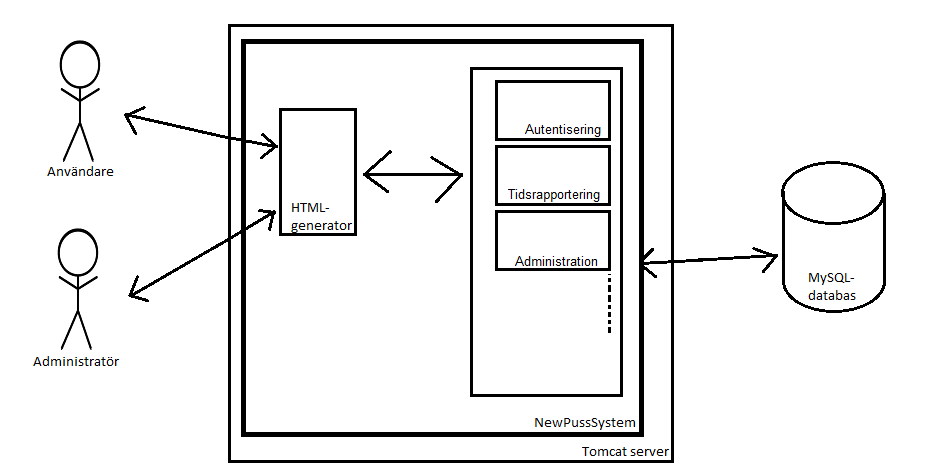
\includegraphics[width=0.75\textwidth]{context}
   \caption{Kontextdiagram för NewPussSystem.}
   \label{image_kontext}
\end{figure}

\section{Funktionella krav}
	\subsection{Generella krav}
		\label{krav-funk-gen}
		\subsubsection*{Övergripande}
		\subsubsection*{Administratör}
		\subsubsection*{Projektledare}
		\subsubsection*{Projektmedlem}
		\subsubsection*{Användare}
		\subsubsection*{Ej inloggad}


	\subsection{Autentisering}
		\label{krav-funk-aut}
		\subsubsection*{Övergripande}
		\subsubsection*{Administratör}
		\subsubsection*{Projektledare}
		\subsubsection*{Projektmedlem}
		\subsubsection*{Användare}
		\subsubsection*{Ej inloggad}
		
	\subsection{Data}
		\label{krav-funk-data}
		\subsubsection*{Övergripande}
		\subsubsection*{Administratör}
		\subsubsection*{Projektledare}
		\subsubsection*{Projektmedlem}
		\subsubsection*{Användare}
		\subsubsection*{Ej inloggad}
		
	\subsection{Administration}
		\label{krav-funk-admin}
		\subsubsection*{Övergripande}
		\subsubsection*{Administratör}
		\subsubsection*{Projektledare}
		\subsubsection*{Projektmedlem}
		\subsubsection*{Användare}
		\subsubsection*{Ej inloggad}

	\subsection{Tidrapportering}
		\label{krav-funk-tid}
		\subsubsection*{Övergripande}
		\subsubsection*{Administratör}
		\subsubsection*{Projektledare}
		\subsubsection*{Projektmedlem}
		\subsubsection*{Användare}
		\subsubsection*{Ej inloggad}


	\subsection{Projektledning}
		\label{krav-funk-proj}
		\subsubsection*{Övergripande}
		\subsubsection*{Administratör}
		\subsubsection*{Projektledare}
		\subsubsection*{Projektmedlem}
		\subsubsection*{Användare}
		\subsubsection*{Ej inloggad}


\section{Kvalitetskrav}
	\subsection{Underhåll}
		\subsubsection*{Övergripande}
		\subsubsection*{Administratör}
		\subsubsection*{Projektledare}
		\subsubsection*{Projektmedlem}
		\subsubsection*{Användare}
		\subsubsection*{Ej inloggad}

	\subsection{Prestanda}
		\subsubsection*{Övergripande}
		\subsubsection*{Administratör}
		\subsubsection*{Projektledare}
		\subsubsection*{Projektmedlem}
		\subsubsection*{Användare}
		\subsubsection*{Ej inloggad}

	\subsection{Användarvänlighet}
		\subsubsection*{Övergripande}
		\subsubsection*{Administratör}
		\subsubsection*{Projektledare}
		\subsubsection*{Projektmedlem}
		\subsubsection*{Användare}
		\subsubsection*{Ej inloggad}

\section{Projektkrav}
	\subsection{Utvecklingsmiljö}
		\subsubsection*{Övergripande}
		\subsubsection*{Administratör}
		\subsubsection*{Projektledare}
		\subsubsection*{Projektmedlem}
		\subsubsection*{Användare}
		\subsubsection*{Ej inloggad}


\end{document}